This chapter will describe the design and implementation of the application which is composed of a representational state transfer (REST) application program interface (API) and a front-end (FE) web application. 

\section{API}
Since the scraped pages of the dark-web were stored via ElasticSearch it was necessary to create a back-end application (BE) in order to perform various operations on the data-set before sending it to the FE. We decided to create a Python BE since the application had to be able to run on a UNIX system. 
\subsection{Technology overview}
Python is a widely used interpreted programming language known for its  readability and portability \cite{aboutPython}. It is open-source and is considered to have an extensive documentation and community available. Another huge advantage is its popularity in the science community. Because of this there is a great amount of useful libraries for research purposes such as NetworkX\footnote{A library used for creating and working with graphs.} \cite{networkX} or cylouvain \footnote{A library with a fast implementation of LA.} \cite{cylouvain}.  
As we wanted to follow the REST architecture we decided to make use of the Django framework \cite{meetDjango}. It is responsible for tasks such as running the server or managing web requests. Another advantage of Django is its Django REST framework (DRF). DRF offers a convenient way for creating restful endpoints and responses. \cite{djangoRest}. Both frameworks are open-source again with extremely helpful documentation and community. 

Because it takes approximately 60 seconds to retrieve about 90,000 pages from the database and circa 13 seconds to divide such a response into communities, caching had to be introduced. For that purpose Redis \cite{redis} is used. It is an open-source solution which we use as a key-value store. It supports  basic data structures as values, e.g. strings, numbers or sets but not custom objects. Since the API uses custom objects for both communities and pages, an object serializer had to be leveraged along with Redis. We decided not to write our own but to utilise the python pickle module \footnote{A module used for converting python objects to streams of bytes and vice versa.} \cite{pickle}. 

\section{Front-end}
For users to be able to see the data acquired from the BE in a reasonable way a FE application was created. 
\subsection{Technology overview}
The probably most favoured programming language used for creating web applications \cite{jsGithut} is called JavaScript (JS) \cite{javaScript}. It is an interpreted language supported by all modern browsers. It is open-source and as such disposes of a big community with splendid documentation. Because it is not strongly typed the code might be complicated to read or navigate. For this reason the FE was written in TypeScript (TS) \cite{typeScript} which is a superset of JS with the advantage of being typed. Both JS and TS come with a significant amount of tools used for implementing user interfaces (UI) in a clean and timely manner. One of the most favoured frameworks is React.js \cite{react} which when used correctly results in readable code and improves performance by managing the re-rendering of page elements.

Since the BE feeds the FE with data which are supposed to be displayed to the user in an interactive way we needed to come up with a mechanism to store this data. We have chosen Redux, a single store approach, to handle this challenge. It fits our architecture perfectly, it is heavily leveraged this way by the React.js community, provides its own set of TS typings and comes with easy to use debugging tools.

The doubtlessly most important part of this FE is the visualization of the graph built on the data sent from the BE. This feature is built using the react-d3-graph library \cite{reactD3Graph} which is 
an implementation of the library d3.js \cite{d3} made more convenient for the use with React.js. 

\subsection{User interface}
After the application is loaded the UI is composed of a header with the name of the application "Dark web categorization" a loader and a sidebar in the right hand side with several inputs or buttons in a column as can be viewed in figure \ref{zeroLevelGraphBasic}. At the very top a drop-down button is present which enables the user to filter the data. Underneath it an input field for filling in a search phrase with a submit button next to it for filtering out a single node or multiple nodes with which the search phrase matches is situated. The last element shown is an indicator of the current level the user is observing which at the beginning is zero. 
\begin{figure}[ht!]
  \centering
  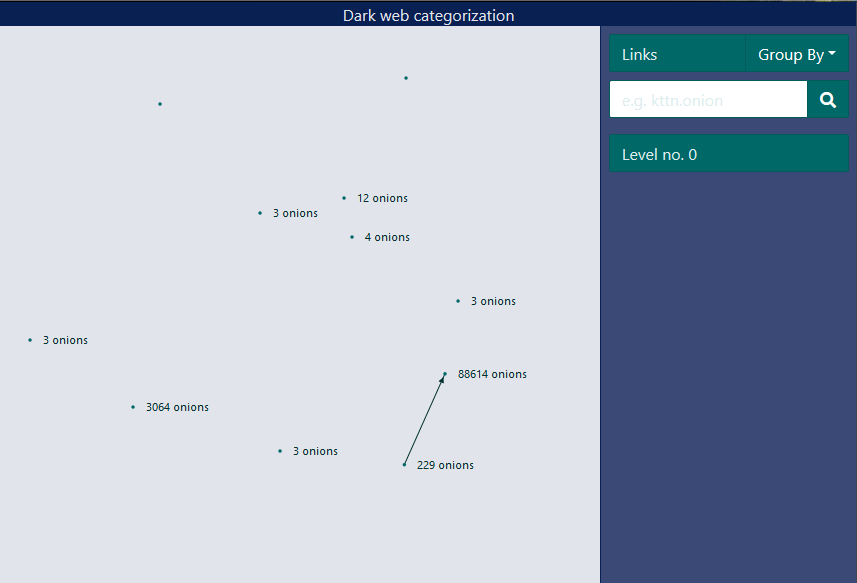
\includegraphics[width=\textwidth]{Images/ZeroLevelGraphBasic.png}
  \caption{The basic view of the app with a selected community and its details.}
  \label{zeroLevelGraphBasic}
\end{figure} 

The moment the data is retrieved from the BE the loader gets replaced for a graph which represents the communities the pages are partitioned into or the pages themselves and the links between them. Each node is displayed as a pie chart of categories of the pages belonging to the community represented by the node (CRN) or the page itself. There also might be a mock-community visible containing isolated nodes which cannot be zoomed into. It is possible for a level to depict communities and pages at once. 

After single-clicking a node additional information is exampled in the sidebar.The details vary depending on whether the node is representing a community or a single page.  
The details of an individual page are as follows: 
\begin {description}
	\item [Url] which also serves as a unique identificator of the page. 
	\item [Category] of the page. Each page belongs to one category.
	\item[Links] to other pages displayed as a list of url addresses. There are up to ten links visible in the sidebar. The remaining links, if any, are downloadable in a text file. 
	\item[Content] of the page if it is available. If the content is too long to be disclosed in the sidebar it is again downloadable in a text file.
\end{description}


The details of a community consist of  grouped information of its pages and include the following:
\begin {description}
	\item [Category composition] which is aggregated from the categories of all the pages of the community. Each category is represented by its name and the percentage of its relevance in the community.
	\item [Page url] addresses (urls) belonging into the community. There are up to ten urls visible in the sidebar. The remaining pages, if any, are downloadable in a text file. 
	\item[Urls count]represents the number of all the pages belonging into the community. 
\end{description}

The CRN needs to be double-clicked in order to zoom into a it to view its sub-communities. If the current level is higher than zero a button for zooming out appears next to the level indicator. It is shown in figure \ref{levelIndicatorWithButton}.
\begin{figure}[ht!]
  \centering
  
\includegraphics{Images/levelIndicatorWithButton.png}
  \caption{The level indicator with the zoom-out button. After the zoom-out button is clicked, the user is shown the communities of the previous level.}
  \label{levelIndicatorWithButton}
\end{figure} 


The user is able to zoom into the very last level (maximum level) where only individual pages are displayed. Each community may have a different maximum level, depending on the number of its pages and its structure.

\subsection{Implementation}
The FE project consists of three folders and several configuration files. The folder \textit{node\_modules} contains imported libraries including React.js, Redux or d3. The next folder named \textit{public} encloses a .ico file \footnote {A picture with the dimensions 16x16 pixels used by the browser to represent the web page or application. It is usually displayed in the tab in which the application is opened.} and a html file which is the default entry point when the application is started. The last folder \textit{src} contains the source code itself. 

As previously mentioned, the FE is written in TS which has the advantage of readability and easy navigation. There are, however, also disadvantages and one of them is the need for every library used is a TS file to be typed. Fortunately typings are downloadable as modules for lots of popular libraries. In case a library has no ready-to-download typings own ones have to be written. In our case the typings for the library react-d3-graph was custom made and can be found in the folder \textit{@types/react-d3-graph}. The file \textit{commont.d.ts} holds types used heavily across the application e.g. Action. The reason for this is not to be liable to import every type every time it is used as types in this file are available for all other files. 

Objects passed between functions in the application have also to be typed. There are three main models

The visual aspect is implemented using Less \cite{less} which is a language extending CSS with improvements such as the possibility of using variables. The Less classes are divided into files according to the elements they are meant to modify and are placed into the folder \textit{styles}. 

The remaining folders each represent a different part of the UI and contain the functionality and the frame of it. The structure of the sub-folders is similar. Therefore it is sufficient to describe them as a whole. Folders named \textit{utils} contain files with helper functions such as converters between server and client models. \textit{Constants} contains folders with string constants or simple functions which return a string depending on the input  of styles and routes. The rest of the folders represent some part of the Redux framework. 

The most basic files which only include string constants are situated in the folders named \textit{actionTypes} which are utilised as action types in actions which are simple objects containing a type and an optional payload. Actions themselves are returned by action creators (AC). AC are functions returning an action and can be found in folders called \textit{actions}. They can be as simple as those present in the file \textit{nodesActionCreators.ts}. But they can be more complicated such as the AC \textit{fetchNodes.ts} and dispatch multiple simple ACs. 

\textit{fetchNodes} and the folder it is placed in share the same name. For easier testing purposes the main logic of this AC is put into a function which receives the simple ACs as dependencies. When this AC is called it first dispatches a simple AC to indicate the fetching has begun. After that an identificator (id) in order to create an error object in case of failure. Next, the fetching itself begins. The fetching in \textit{fetchNodes} is realized with the library isomorphic-fetch. The fetch function of this library expects the first argument to be the url address to the resource. The second argument is an object describing further details of the request and is optional. For instance the request method, headers or the payload. If the request does not result in error the response status is checked. After the fetching is complete the node-mode is updated depending on whether communities were acquired or the maximum level was reached and the response contains only individual pages. Afterwards a success AC with the response is dispatched. If an error is caught during the fetching a failure AC with the previously created error id is dispatched.

The dispatching of actions enables the changing of the state via reducers situated in the \textit{reducers} folders. The state is a single object for the whole application and is immutable \footnote{The object cannot be adjusted directly. Instead, a new modified object is returned and the original one stays unmodified.}. A reducer is a pure function \footnote{The return value of a pure function is only dependent on its input values. A pure function has no side effects.} receiving the current state with the dispatched action as its arguments and returning the newly computed state. A reducer creates a new state only if it recognizes the type of the given action. If not, the old state is returned. Because the state is immutable and every returned object would change the whole state the function \textit{combineReducers} is leveraged. It expects an object containing reducers as its argument. It achieves performance adjustments so that the state is modified only when there have been valid changes.

The folders \textit{components} contain files with React components. They represent the skeleton of the UI with the specified behaviour. 

